\section{Evolution of cameras}
"A camera is an optical instrument that captures a visual image.
The camera body has a small hole (the aperture) that allows light through to capture an image on a light-sensitive surface (usually photographic film or a digital sensor). Lenses focus the light entering the camera, and the size of the aperture can be widened or narrowed. A shutter mechanism determines the amount of time the photosensitive surface is exposed to light"~\cite{cameraWiki}.
The invention of the camera has been traced back to the work of Alhazen (Ab\={u} `Al\={i} al-\d{H}asan ibn al-\d{H}asan ibn al-Haytham). Alhazen invented the pinhole camera \emph{camera obscura}, and explained its scientific principles in his magnum opus \textit{Book of Optics} (\textit{Kit\={a}b al-Man\={a}\d{z}ir}) in the 11\textsuperscript{th} century AD~\cite{al2015retrospect}. 
The camera obscura was originally used for viewing solar eclipses instead of looking directly at the sun and damaging the eye.

\begin{figure}[hb]
    \centering
    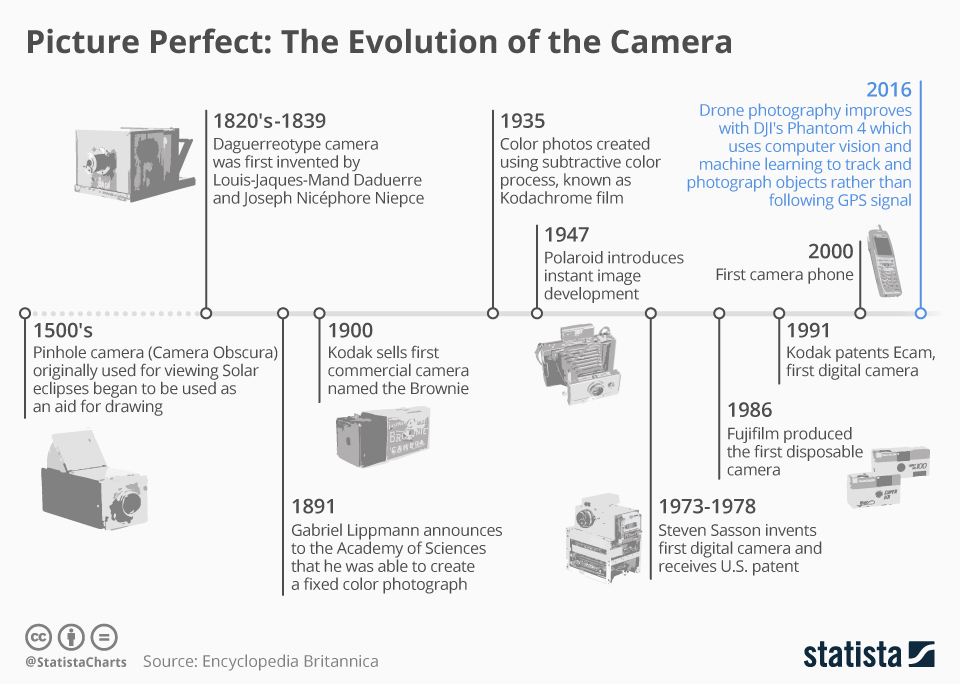
\includegraphics[width=\textwidth]{Figures/camera_timeline.jpeg}
    \caption{The evolution of the camera~\cite{statista2019camera}.}
    \label{fig:CameraEvolution}
\end{figure}

The camera has evolved over the last millennium in technology, functionality and versatility. 
A brief overview of the evolution of the camera (that uses visible light) is illustrated in Fig.~\ref{fig:CameraEvolution}.
Artists used the first pinhole cameras to draw the outline of their paintings from real landscapes.
Then, the cameras were used to preserve memories and store the image information in a physical format.
The landmark moment was the invention of the digital camera, where the image is recreated from the light falling on a \gls{ccd} instead of a photographic film.
The first digital camera was invented by Llyod and Sasson in 1975 and patented in 1978~\cite{lloyd1978electronic}. 
However, at that time, it did not gain the necessary recognition it deserved~\cite{estrin2015Kodak} due mostly to managerial decisions.
One of the reasons for non-acceptance was that it took 23 seconds to record a captured image into a cassette tape (for storage).
The first professional digital \gls{slr} camera was created by Sasson and Hills in 1989 and patented in 1991~\cite{sasson1991electronic}. 
"It had a 1.2 megapixel sensor, and used image compression and memory cards"~\cite{estrin2015Kodak}.

\begin{figure}[ht]
    \centering
    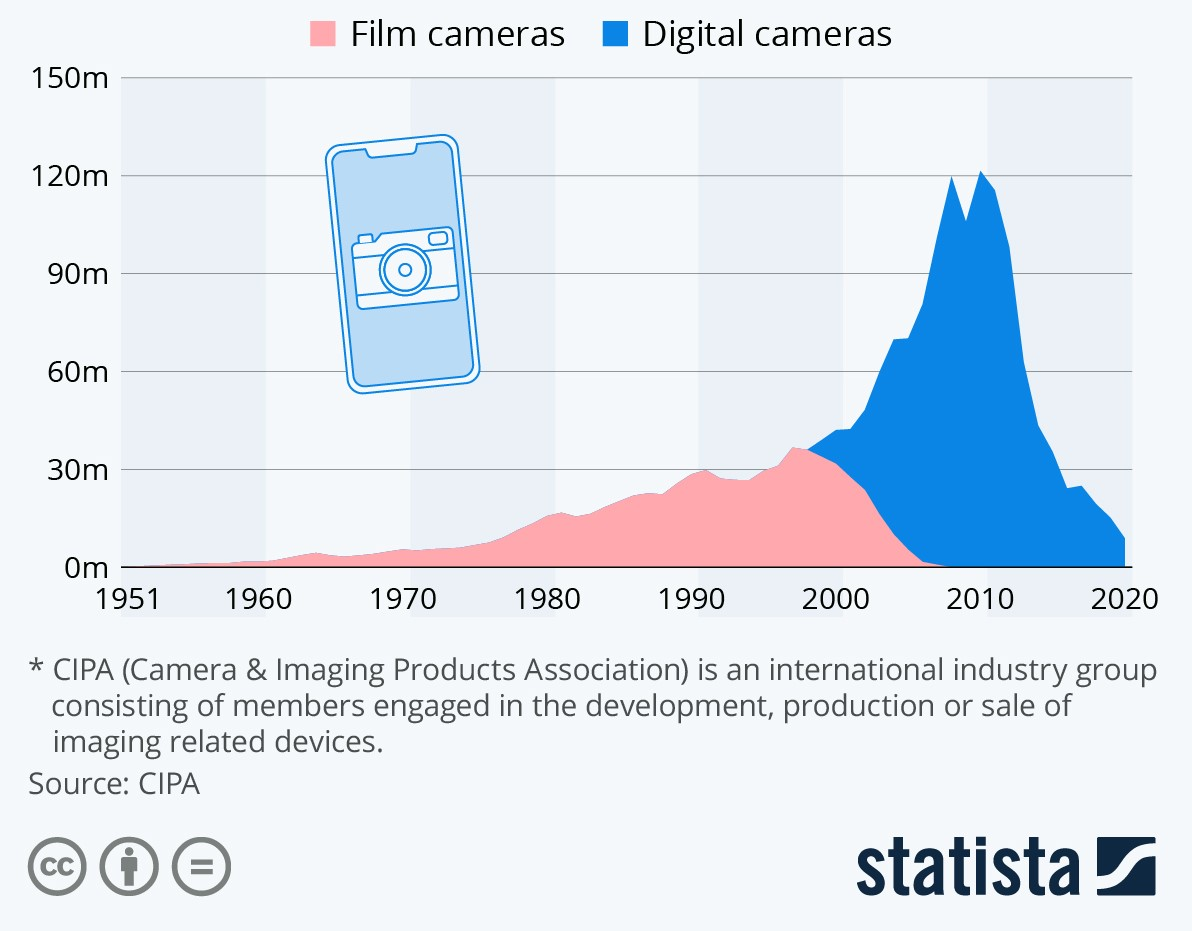
\includegraphics[width=0.7\textwidth]{Figures/camera2.jpeg}
    \caption{Worldwide shipments of photo cameras~\cite{statista2021camera}.}
    \label{fig:CameraSales}
\end{figure}

The invention of the professional digital camera revolutionised the camera market and also increased the global camera market size and revenue. 
The growth of photo camera sales is illustrated in Fig.~\ref{fig:CameraSales}.
Two interesting points to note are: (i) the domination of digital cameras over film cameras that wiped out the normal use of film cameras; and (ii) the drastic decline in sales of digital photo cameras.
The latter is due to the advancements in technology and the integration of high-quality cameras in smartphones and tablets. 
Buying a modern smartphone with a high-quality camera is generally preferred over a single-purpose photo camera. 

\begin{sloppypar}
Advancements in low-cost \gls{cmos} image-sensor technology~\cite{el2005cmos} and Moore's law~\cite{moore1998cramming} enabled the faster integration of cameras in smartphones and modern industrial systems.
Moore's law predicted that the number of transistors in integrated circuits would double every two years, and this has been happening over the last many decades.
This enabled the miniaturisation of the size of the semiconductor component.
Alternatively, many more \gls{cmos} sensors, processors and memories can be densely packed into a semiconductor component of the same size.
This reduced the overall cost and size of the camera, thus enabling the widespread use of cameras in smartphones, laptops, security devices, video surveillance, drones, autonomous systems, modern industrial systems, and so on.
For instance, the latest Samsung Galaxy S21 FE 5G smartphone has four cameras - a 12MP ultra-wide camera, a 12MP wide-angle camera, an 8MP telephoto camera, and a 32MP selfie camera~\cite{samsungS21}.
\end{sloppypar}

\begin{figure}[ht]
    \centering
    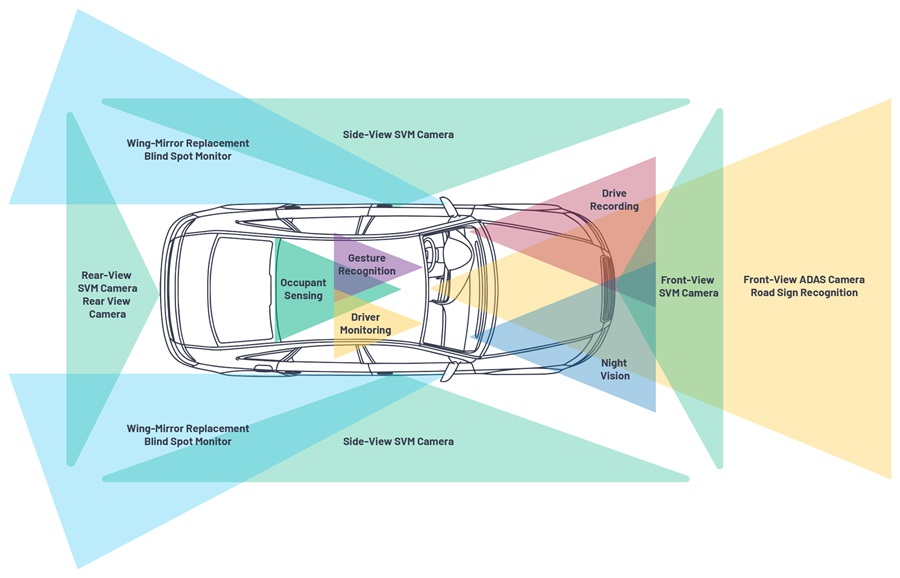
\includegraphics[width=\textwidth]{Figures/295762-fig-01.jpg}
    \caption{Proliferation of cameras in modern vehicles~\cite{triggs2020camera}.}
    \label{fig:CameraProliferation}
\end{figure}

The latest Tesla autopilot system has eight cameras~\cite{tesla}, which are necessary for the three-dimensional perception of the surrounding environment~\cite{elluswamy2021predicting}.
In the automotive domain, there is an immense proliferation of cameras in modern vehicles (illustrated in Fig.~\ref{fig:CameraProliferation}).
According to an industrial report from Yole~\cite{yole19}, the number of cameras in a single vehicle is expected to grow even further. Yole estimates 11 cameras per vehicle by 2024 for functionalities like surround-view, \glspl{adas}, night vision, e-mirror replacement and driver monitoring.
Yole predicts that cameras would also be an integral part of fully autonomous systems.
Additionally, different types of cameras (based on the wavelength of light) are gaining significance for varied purposes, such as hyperspectral cameras~\cite{behmann2018specim}, thermal-imaging cameras~\cite{lee2018analyzing} (using infrared light) and laser imaging (used in lidar sensors~\cite{li2020lidar}). 
Cameras have thus proven to be irreplaceable for modern applications and systems in the coming decades.